\documentclass{article}
\usepackage[top=25truemm,bottom=20truemm,left=20truemm,right=20truemm]{geometry}

\usepackage{amsmath}
\usepackage{amssymb}
\usepackage{amsfonts}
\usepackage{mathrsfs}
\usepackage{latexsym}
\usepackage{bm}
\usepackage[dvipdfmx]{graphicx}


\title{Notes on topic in which I am interested}
\author{Ryota Masuki}
\date{\today}

\begin{document}
\maketitle

\section{Section 1}
\begin{align}
    a = b\times c
\end{align}
\begin{table}
    \begin{center}
      \caption{FRUITS}
     \begin{tabular}{lrr}
       Topic & Price(Euro) & Number \\
       Apple & 100 & 5 \\
       Orange & 50 & 10
     \end{tabular}
    \end{center}
   \end{table}

   \begin{figure}[htbp]
    \begin{center}
    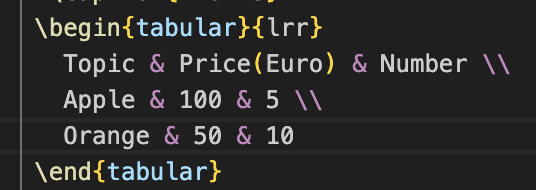
\includegraphics[width=100mm]{screenshot.png}
    \caption{screenshot}
    \end{center}
    \end{figure}
    
   \end{document}